\chapter{Cours 1}
\section{Introduction}
Le nombre des transistor sur les circuits intégrés double tous les 18 mois. Si on continue
ainsi, les transistor auront atteint la taille d'un atome d'hydrogène d'ici 2030. On ne
peut plus échapper à une vision quantique de la théorie de l'information.\\

La \textit{théorie quantique} (début 1900), pour les physiciens, cherche à comprendre 
la matière à l'échelle atomique. D'autre part, la \textit{théorie de l'information}
(début 1940), pour les ingénieurs, cherche à caractériser l'information et à élaborer des
moyens de communications. L'union des deux a donné naissance à la \textit{théorie de 
l'information quantique}, où l'on a développé un équivalent quantique aux notions 
classiques
\begin{center}
Quantum bits, quantum logic gates, quantum circuit,  quantum computer, \dots
\end{center}
Cette théorie concerne à la fois les physiciens \textit{et} les ingénieurs quantiques.
La motivation de l'ingénieur consiste à pousser les limites de la théorie de l'information
quantique (des ordinateurs qui peuvent résoudre des problèmes difficiles, des moyens
de communications basés sur la téléportation, un codage dense et de nouvelle techniques
de cryptographie). Pour le physicien, c'est un nouveau champ passionnant (par exemple,
la téléportation quantique théorisée en 1933 et démontrée en 1998).\\

Certains dispositifs basés sur des applications quantiques existent déjà aujourd'hui. 
La compagnie \textit{ID Quantique} (Genève) commercialise un processus de cryptage
des fibres optiques.\\

\textbf{Outlines of this course}
\begin{itemize}
\item[$\bullet$] De la théorique classique à quantique.
\item[$\bullet$] Qu'est ce qui est vraiment spécial aux qbit (optiques) ? Application :
algorithmes quantiques.
\item[$\bullet$] Qu'est ce qui est si spéciale à l’intrication ? Application : 
téléportation quantique.
\end{itemize}
\newpage
\section{Théorie de l'information : du classique au quantique}
\subsection{Commençons classiquement : Shannon}
La technologie actuelle se base sur la théorie de l'information élaborée par 
\textsc{Shannon} (1948 et 1949). Elle se base sur deux grands principes :
\begin{description}
\item[Mesure de l'information] Chaque type d'information (texte, image, son) peut être 
associé à un \textbf{contenu d'information}, qui quantifie avec quelle efficacité
elle peut être représentée par des 0 et 1.
\item[Limite sur les communications] Tout canal de communication imparfait (téléphone, 
radio, satellite) à une \textbf{capacité} qui quantifie la quantité d'information qui 
peut être transmise correctement sur un canal.
\end{description}

\subsubsection{Source coding theorem (codage sans bruit)}
Le plus grand taux de compression des données pour une source est donnée par 
l'\textbf{entropie de Shannon} $H=f($statistique de la source$)$.
\begin{equation}
01\text{\st{1}}010\text{\st{01}}110\text{\st{10}}01\quad\Rightarrow\quad 01|010|110|01
\end{equation}
$\to$ Faire un "\textit{code source}", c'est supprimer la redondance

\subsubsection{Channel coding theorem (codage bruité)}
Le plus grand taux de transmission possible via un canal est donné par la 
\textbf{capacité de Shannon} $C=f($statistique du bruit$)$.
\begin{equation}
0101011001\quad\Rightarrow\quad 011010011101001
\end{equation}
$\to$ Faire un "\textit{code correcteur d'erreur}", c'est ajouter de la redondance.


\exemple{\textsc{source coding}.\\
La \textit{source} est une variable aléatiore définie par
\begin{equation}
p(x) = \left\{\begin{array}{ll}
1/2&x=A\\
1/4&x=B\\
1/8&x=C\\
1/8&x=D
\end{array}\right.
\end{equation}
On lui associe le codage simple $A\to00, B\to 01, C\to 10, D\to 11$. Ainsi, $L=2$ bits par
symbole. On peut calculer l'entropie
\begin{equation}
H(X) = -\sum_{x=A}^D p(x)\log_2p(x) = \frac{1}{2}+\frac{2}{4}+\frac{3}{8}+\frac{3}{8}=
\frac{7}{4}<2
\end{equation}
La longueur moyenne d'un code $L$ est supérieure où égale à l'entropie
\begin{equation}
L \geq H(X)
\end{equation}
Avec un codage plus intelligent, on peut saturer la précédente inégalité. Le codage
$A\to0,B\to10,C\to110,D\to111$ donne
\begin{equation}
L := \frac{1}{2}*1+\frac{1}{4}*2+\frac{1}{8}*3+\frac{1}{8}*3=\frac{7}{4}<2
\end{equation}
Ici, $L=7/4$ bits par symbole.}
\subsection{Information et physique}
Rolf \textsc{Landauer} a donné de fortes implications liée au fait que l'\textbf{information
est physique}. Il en découle deux grands principes
\begin{description}
\item[Il n'y a pas d'information sans représentation] Chaque bit d'information doit être
transporté par un \textit{système physique}, ce n'est pas un concept immatériel.
\item[Il n'y a pas de traitement sans processus] Chaque traitement de l'information doit
être réalisé par un \textit{processus physique.}
\end{description}

\subsubsection{Information de thermodynamique}
Stocker un bit à un coût thermodynamique du à l'irréversibilité. Si l'on cherche à décrire
un calcul classique, il sera irréversible et va ainsi dissiper de l'énergie. Par exemple, 
quand on veut effacer de l'information c'est quelque chose d'irréversible, qui coûte donc
de l'énergie. On s'intéresse ici à l'effacement de "010010101110101001000101", qui correspond 
à une température $T$. On veut le changer en "0000000000000000000000", correspondant à une
température 0.\\

\cadre{\textsc{Principe de Landauer}\ \\
Le coût thermodynamque de l'effacement d'un bit est (en joules)
\begin{equation}
\ln(2)kT
\end{equation}
C'est un processus \textit{irréversible}.}\ 

La notion d'un ordinateur classique réversible est précurseur à la notion de codage quantique.




\subsubsection{Logique réversible et irréversible}
	\begin{wrapfigure}[12]{l}{8.5cm}
	\vspace{-5mm}
	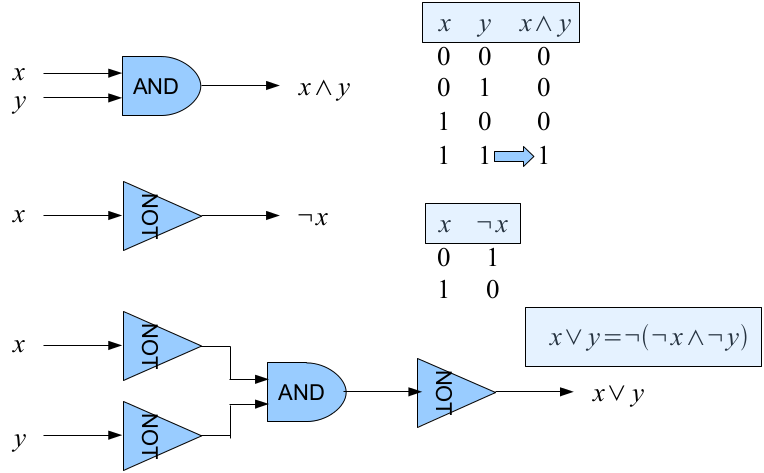
\includegraphics[scale=0.3]{ch1/image1.png}
	\captionof{figure}{ }
	\end{wrapfigure}
Ci-contre, les plus connues de portes logiques. La porte \textit{AND} est irréversible car si 
la sortie est 0, il n'est pas possible de savoir quel était l'entrée. Par contre la porte
\textit{NOT} est réversible (on peut connaître l'entrée avec la sortie). La dernière est 
une composition des deux dernières portes avec une irréversibilité. Il s'agit d'une porte
\textit{OR}. Ceci signifie que l'on va dissiper de l'énergie à un moment donné. \textbf{Les portes
\textit{AND} et \textit{NOT} forment un ensemble universel de portes irréversibles}. \\

	\begin{wrapfigure}[10]{r}{8cm}
	%\vspace{-5mm}
	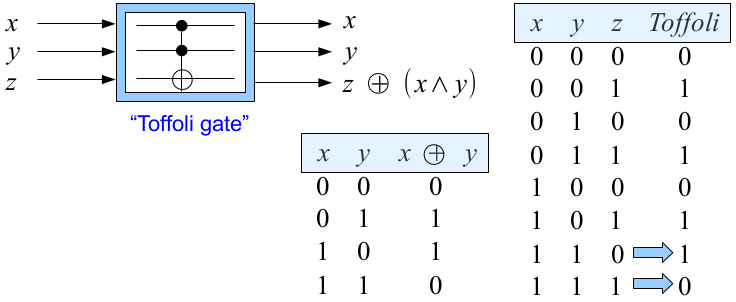
\includegraphics[scale=0.3]{ch1/image2.png}
	\captionof{figure}{ }
	\end{wrapfigure}
	
Pour créer un porte universelle réversible, il faut avoir 3 bits. Si on parvient à faire 
quelque chose de totalement réversible, on pourrait créer un ordinateur sans coût ni énergie. La
porte \textit{Toffoli} copie $x$ et $y$ puis, pour $z$ 
\begin{equation}
z \to z\oplus(x\wedge  y)
\end{equation}
On peut voir $x\oplus y$ comme $\mod_2(x+y)$ (voir tableau ci-contre). Il s'agit du \textit{NOT
EXCLUSIF}. Si $x$ \textbf{et} $y$ valent 1, on effectue $NOT\ z$. Sinon, on copie $z$.
On peut prouver que cette porte est suffisante pour implémenter chaque porte logique,
elle est universelle. On a pensé que c'était le futur des ordinateurs car ils ne dissipent 
aucune énergie, mais on ne savait pas l'implémenter. C'est la première étape vers les ordinateurs
quantiques. On a quelque chose d'universel et maintenant, on veut aller vers le quantique.


\section{Information et physique quantique}
Qu'est ce qui se passe si l'on encode l'information dans les états d'un système quantique ? 
N'importe quel système à deux niveaux (spin, polarisation des photons, \dots) peut être 
utilisé pour faire un qbit. Alors qu'un bit ne peut prendre que 0 et 1 comme valeur, un 
qbit peut être dans une superposition.
\begin{equation}
\alpha\ket0+\beta\ket1
\end{equation}
Cela signifie qu'il peut exister dans n'importe quel état combili de deux. Chaque état qbit
peut être représenté par un vecteur dans une sphère. On peut ainsi être "entre le mode 
\textit{on} et \textit{off}" pour lequel il n'existe pas d'équivalent classique. La superposition
n'est \textbf{pas} une mixture probabilistique (parfois 1, parfois 0). Si l'on a une superposition
pour des milieurs de particules, on parlera d'intrication (plus qu'une corrélation classique).\\

Les qbits optiques sont des photons. Si on a une onde plane, on peut lui associer une polarisation
linéaire. Si la polarisation est horizontale, c'est $\ket 0$ et si elle est verticale $\ket 1$. Un
photon et son état de polarisation transporte un qbit. Il peut avoir une polarisation diagonale
(45$^\circ$) via superposition quatique
\begin{equation}
\ket0+\ket1
\end{equation}
C'est bien le résultat d'une superposition et \textbf{pas} "parfois vertical, parfois horizontal". 
C'est un photon qui a une polarisation le long de la diagonale. En mesurant on aura l'un ou l'autre,
mais avant il s'agit clairement d'une superposition.\\

Avec un McZehnder, un faisceau peut être spatialement séparé en deux. L'onde réfléchie gagne une
phase de $\pi/2$ et il y a deux sorties possibles : l'une verra des interférence constructives,
l'autre destructives (gauche). Diminuons l'intensité de la source pour n'avoir plus que un photon (ça existe!). A priori, si on envoie un photon, on ne devrait pas avoir de détection la ou il y avait des
interférences destructives (centre). Si on mesure avec deux détecteurs, on n'a jamais de superposition :
clic à gauche ou à droite (probabilité $1/2$), mais pas les deux (droite). Ceci montre qu'il n'y a 
qu'un seul photon dans l'interféromètre.

\begin{center}
	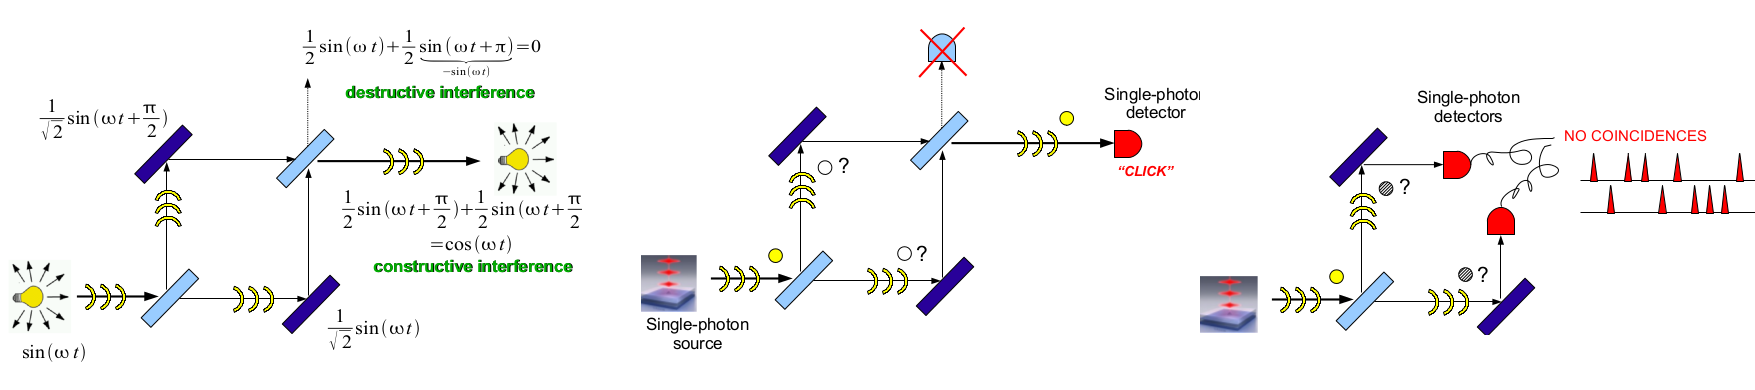
\includegraphics[scale=0.25]{ch1/image3.png}
	\captionof{figure}{ }
\end{center}
\newpage
D'un point de vue physique \textbf{classique}, le photon est toujours détecté dans le même détecteur
et ce peu importe le chemin qu'il emprunte comme le montre l'image ci-dessous
\begin{center}
	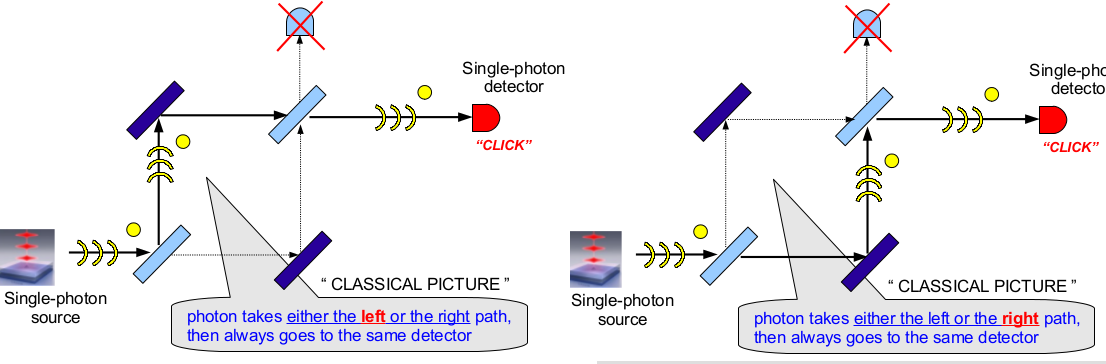
\includegraphics[scale=0.3]{ch1/image4.png}
	\captionof{figure}{ }
\end{center}

Insérons maintenant une lame de phase. Sa présence fait que ça interfère et l'on a maintenant des
clic à l'autre détecteur (gauche). D'un point de vue \textbf{classique}, le clic est indépendant
du chemin suivi. Un photon qui va tout droit va traverser la lame de phase et provoquer un clic
dans le détecteur du haut (centre). Toujours classiquement, un photon qui prend le chemin de 
gauche doit aussi faire un clic sur le détecteur du haut (droite), mais \textbf{comment un photon du
chemin de gauche peut-il sentir la lame de phase du "chemin droit"} ? 

\begin{center}
	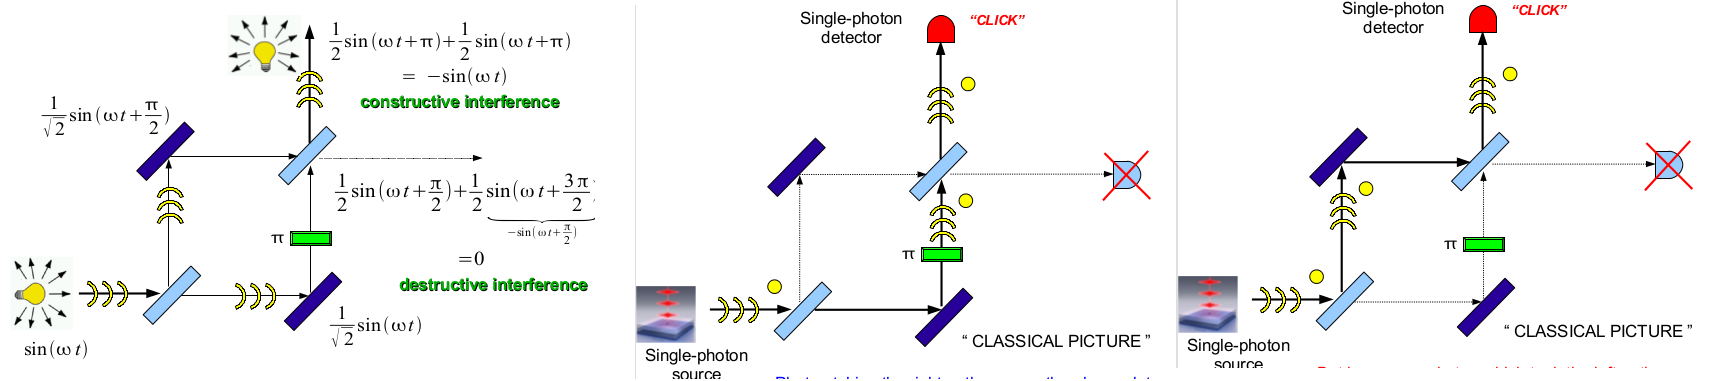
\includegraphics[scale=0.25]{ch1/image5.png}
	\captionof{figure}{ }
\end{center}

C'est possible par \textbf{dualité}. Le photon n'est pas "à gauche ou à droite", mais dans une
superposition entre les deux.
\begin{center}
	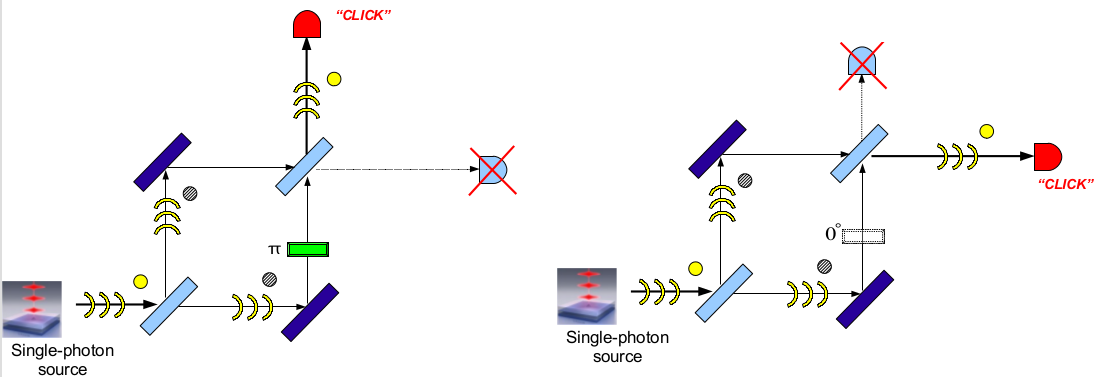
\includegraphics[scale=0.3]{ch1/image6.png}
	\captionof{figure}{ }
\end{center}

\newpage
\subsection{Dans un langage quantique}
	\begin{wrapfigure}[7]{l}{8cm}
	\vspace{-5mm}
	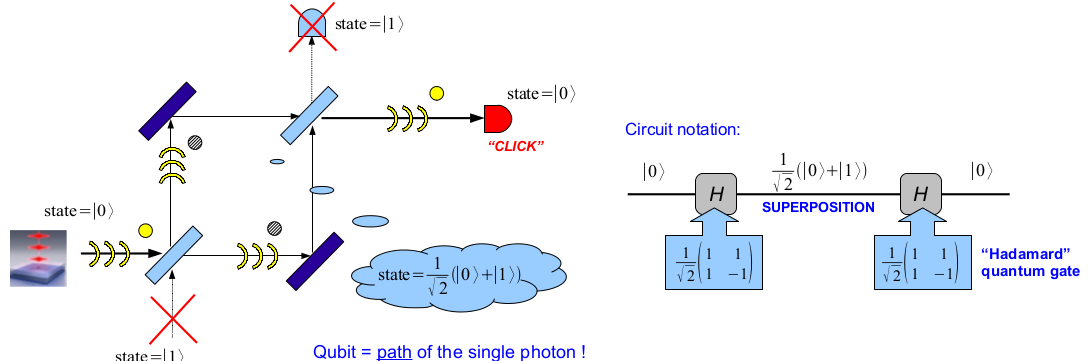
\includegraphics[scale=0.2]{ch1/image7.png}
	\captionof{figure}{ }
	\end{wrapfigure}
Dans l'interféromètre, entre les deux beamspliter, on peut noter l'état comme une superposition
\begin{equation}
\frac{1}{\sqrt{2}}(\ket0+\ket1)
\end{equation}
Le \textbf{qbit est le chemin d'un unique photon}. Adoptons la notation mathématique des
vecteurs d'états (vecteurs complexes de dimension deux dans l'espace d'Hilbert)
\begin{equation}
\ket0\equiv\left(\begin{array}{c}
1\\
0
\end{array}\right)\qquad\qquad\ket1\equiv\left(\begin{array}{c}
0\\
1
\end{array}\right)
\end{equation}
On peut transcrire le McZehnder en circuit à l'aide des portes d'\textsc{Hadamard}
\begin{equation}
H = \frac{1}{\sqrt{2}}\left(\begin{array}{cc}
1&1\\
1&-1
\end{array}\right)
\end{equation}
En effet, nous partons de $\ket0$ et nous passons la première porte (beamsplit)
\begin{equation}
H\ket0 = \frac{1}{\sqrt{2}}\left(\begin{array}{cc}
1&1\\
1&-1
\end{array}\right)\left(\begin{array}{c}
1\\
0
\end{array}\right)=\frac{1}{\sqrt{2}}\left(\begin{array}{c}
1\\
1
\end{array}\right) = \frac{1}{\sqrt{2}}(\ket0+\ket1)
\end{equation}
Il s'agit d'une superposition quantique. Ici, la probabilité d'avoir l'un ou l'autre
(mesure) est de $1/2$.L'état $\frac{1}{\sqrt{2}}(\ket0+\ket1)$ passe alors la seconde porte 
(deuxième BS)
\begin{equation}
H\left[\frac{1}{\sqrt{2}}(\ket0+\ket1)\right] = 
\frac{1}{\sqrt{2}}\left(\begin{array}{cc}
1&1\\
1&-1
\end{array}\right)\frac{1}{\sqrt{2}}\left(\begin{array}{c}
1\\
1
\end{array}\right) =\left(\begin{array}{c}
1\\
0
\end{array}\right)=\ket0
\end{equation}
Nous avons bien décrit la situation de la figure 1.7, dans un langage quantique.

\subsection{Parallélisme quantique}
	\begin{wrapfigure}[8]{l}{5cm}
	\vspace{-5mm}
	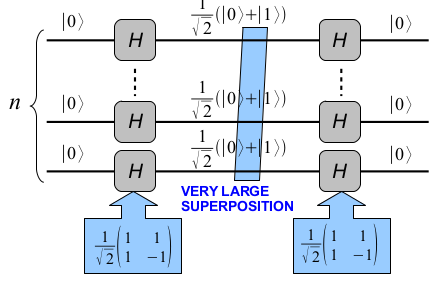
\includegraphics[scale=0.29]{ch1/image8}
	\captionof{figure}{ }
	\end{wrapfigure}
On aimerait cette fois avoir tous les états en même temps. A l'entrée et à la sortie, 
nous n'avons toujours que des $\ket0$. Entre les deux, c'est plus intéressant : nous avons
une superposition qui donne un nombre exponentiel de terme. Avec seulement $n$ qbits, on
peut obtenir l’entièreté de $\mathcal{H}$. Chaque qbit à la même histoire, mais l'état 
joint peut être décrit comme une superposition exponentielle de $2^n$ états pour $n$
qbits. Par exemple, si $n=3$ :
\begin{equation}
(\ket0+\ket1)(\ket0+\ket1)(\ket0+\ket1)=\underbrace{\ket0\ket0\ket0}_{'0'}+
\underbrace{\ket0\ket0\ket1}_{'1'}+\underbrace{\ket0\ket1\ket0}_{'2'}+\dots+
\underbrace{\ket1\ket1\ket1}_{'7'}
\end{equation}


\newpage
\subsection{Intrication quantique}
	\begin{wrapfigure}[5]{l}{5cm}
	\vspace{-5mm}
	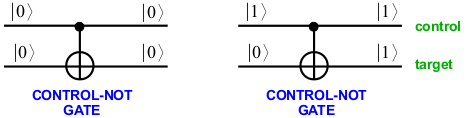
\includegraphics[scale=0.29]{ch1/image9}
	\captionof{figure}{ }
	\end{wrapfigure}
Ci-contre, une porte \textit{CONTROL-NOT}. Il s'agit d'une porte qui agit sur deux bits (l'idée
est la même que la porte sans pertes à 3 bits). Le qbit supérieur est celui de \textit{contrôle},
il ne change pas. En dessous, c'est le qbit \textit{cible} qui est inversé (\textit{NOT}) si le
qbit de contrôle est $\ket 1$ (\textit{CONTROL}).\\

	\begin{wrapfigure}[5]{r}{5cm}
	\vspace{-5mm}
	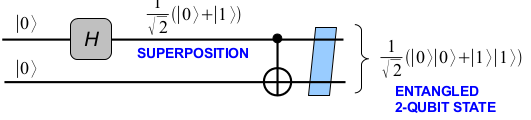
\includegraphics[scale=0.29]{ch1/image10}
	\captionof{figure}{ }
	\end{wrapfigure}
Le contrôle dit s'il faut inverser la cible, mais que se passe-t-il si le contrôle est une 
superposition quantique de ses deux états possibles? Si $\ket0$ ça change rien, mais si 
$\ket1$ (contrôle) alors il faut que $\ket0\to\ket1$ (cible). Le nouvel état de sortie peut 
être écrit
\begin{equation}
\frac{1}{\sqrt{2}}\left(\ket0\ket0+\ket1\ket1\right)
\end{equation}
Cet état est intéressant car même si on change de base ($\ket0,\ket1$ n'est qu'un choix)
on ne sera jamais capable d'écrire cet état de sortie comme un produit. Il est dit 
\textbf{intriqué} : il n'est pas possible d'écrire chaque qbit séparément, on doit l'écrire
comme tel.\\

\retenir{On peut construire n'importe quel circuit quantique en combinant la porte d'
\textsc{Hadamard} $H$ et une porte quantique à 2-qbit (comme ci-dessus).
\begin{center}
Circuit quantique = \{Porte quantique à 1-bit, Portes quantique à 2-bit\}
\end{center}
Ceci donne lieux à des états à $n$-qbit fortement intriqués. Pas besoin d'avoir
3 qbits ici.}


\subsection{Circuit quantique (exemple)}
	\begin{wrapfigure}[8]{l}{5.5cm}
	\vspace{-5mm}
	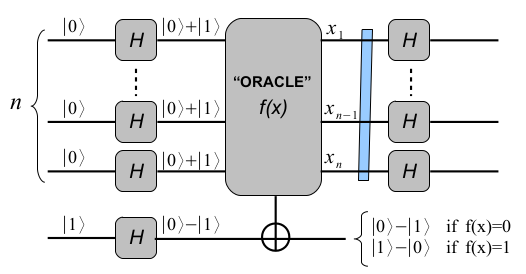
\includegraphics[scale=0.3]{ch1/image11}
	\captionof{figure}{ }
	\end{wrapfigure}
Nous avons un \textbf{oracle} $f(x)$, une boîte noire. Le but de l'algorithme est de dire
ce que faire l'oracle de façon quantique en explorant toutes ses entrées possibles en même temps.
Nous savons que nous aurons à la superposition de toutes les possibilités. Ainsi, le
vecteur $x$ est la superposition de toutes les entrées possibles !\\

D'abord, le vecteur $x$ est copié (à droite de l'oracle). Ensuite, l'oracle va inverser le 
qbit $(n+1)$ si $f(x)=0$ ou $f(x)=1$. C'est comme ça qu'on défini l'oracle (c'est une sorte
de grosse porte \textit{CTRL-NOT}). 
\begin{equation}
\ket0-\ket1 \quad\Rightarrow\quad \left\{\begin{array}{ll}
\ket0-\ket1&\text{si }f(x)=0\\
\ket1-\ket0&\text{si }f(x)=1
\end{array}\right.
\end{equation}
On peut réécrire ce "flip" comme un facteur de phase. Avant la seconde porte 
d'\textsc{Hadamard} (rectangle bleu), on a alors l'état suivant
\begin{equation}
\sum_{\vec{x}=00\dots0}^{11\dots1} (-1)^{f(\vec x)}\ket{x_1}\ket{x_2}\dots\ket{x_n}\left(
\ket0-\ket1\right)
\end{equation}
La somme est présente car nous avons bien toutes les possibilités d'entrées. Pour voir
ce qui se passe après la deuxième "colonne de $H$", remarquons que nous pouvons réécrire
la porte d'\textsc{Hadamard} de la façon suivante
\begin{equation}
\left.\begin{array}{ll}
H\ket0 &=\frac{1}{\sqrt{2}}(\ket0+\ket1)\\
H\ket1 &=\frac{1}{\sqrt{2}}(\ket0-\ket1)
\end{array}\right\}\quad\Rightarrow\quad H\ket x=\frac{1}{\sqrt{x}}\sum_{y=0}^1(-1)^{xy}\ket y
\end{equation}
En utilisant cette dernière relation, on obtient en sortie
\begin{equation}
\sum_{\vec{x}=00\dots0}^{11\dots1} (-1)^{f(\vec x)}\underbrace{\sum_{\vec{y}=00\dots0}^{11\dots1} (-1)^{
\vec{x}\vec{y}}\ket{y_1}\ket{y_2}\dots\ket{y_n}}_{\text{Effet des $H$ sur } \ket{x_1}
\ket{x_2}\dots\ket{x_n}}
\end{equation}
où $\vec{x}\vec{y} = x_1y_1+x_2y_2+\dots +x_ny_n$. Échangeons les deux sommations
\begin{equation}
\sum_{\vec{y}=00\dots0}^{11\dots1} \left[\sum_{\vec{x}=00\dots0}^{11\dots1} (-1)^{f(\vec{x})+
\vec{x}\vec{y}}\right]\ket{y_1}\ket{y_2}\dots\ket{y_n}
\end{equation}
Nous avons maintenant une somme sur $\vec{y}$ pondérée par un coefficient qui donnera la 
probabilité d'amplitude de chaque sortie possible (entre crochets). Après mesure, nous
aurons des 0/1.

\subsection{Algorithme quantique (Deutsch-Josza)}
L'idée principale de savoir si nous avons une fonction $f(x)$ constante ou \textit{balanced}. 
Nous avons $f(x)$ et nous voulons savoir quelque chose sur lui en minimisant le nombre de
requête.

\subsubsection{Fonction constante}
	\begin{wrapfigure}[4]{r}{3.5cm}
	\vspace{-5mm}
	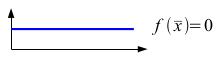
\includegraphics[scale=0.5]{ch1/image12}
	\captionof{figure}{ }
	\end{wrapfigure}
Si la fonction est constante, on remplace $f(\vec{x})$ par zéro. L'amplitude de probabilité devient
\begin{equation}
\left[\sum_{\vec{x}=00\dots0}^{11\dots1} (-1)^{
\vec{x}\vec{y}}\right]=0
\end{equation}
\textbf{Sauf si} $y_1=y_2=\dots=0$. On peut la réécrire
\begin{equation}
\underbrace{\sum_{x_1=0}^1(-1)^{x_1y_1}}_{y_1=0}\underbrace{\sum_{x_2=0}^1(-1)^{x_2y_2}}_{y_2=0}\dots
\end{equation}
On mesurera alors toujours $000\dots0$ (seul état de probabilité non nulle).

\subsubsection{Fonction "balanced"}
	\begin{wrapfigure}[4]{r}{3.5cm}
	\vspace{-5mm}
	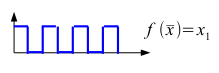
\includegraphics[scale=0.5]{ch1/image13}
	\captionof{figure}{ }
	\end{wrapfigure}
Dans ce cas (autant de 0 que de 1), nous avons $f(\vec{x})=x_1$. En remplaçant
\begin{equation}
\left[\sum_{\vec{x}=00\dots0}^{11\dots1} (-1)^{x_1+
\vec{x}\vec{y}}\right]=0
\end{equation}
\textbf{Sauf si} $y_1=1, y_2=\dots=y_n=0$. On va alors mesurer $100\dots0$.\\

En \textbf{un seul appel}, on peut distinguer si on a une fonction constante ou balancée (grâce au
parallélisme quantique). En mesurant la sortie, on peut directement savoir ça. Classiquement, dans
le pire des cas, il faudrait faire au moins la moitié de toutes les entrées\footnote{Voir schéma
notes} pour s'assurer qu'il n'y a pas de montée (elle serait alors constante) ce qui demanderait
$2^n/2=2^{n-1}$ appels! On comprend ici l'intérêt de l'algorithme quantique.


\iffalse

Fct cste
L’aplitude de proba est donnée par ça. On remplace f par 0.  On peut la réécrire (voir notes). Si la foncition est nulle, on mesurera toujours 0000 car les autres bits ont une proba nulle d’être détectée. 



Balanced function
Même idée mais un +x1.  On va mesurer 1 au premier et 0 partout ailleurs 
En un seul appel on peut distinguer si on a une fonction constante ou balancée.  Simplement en mesurer la sortie on peut savoir si on a une fct constante ou balancée. Alors que classiquement il faudrait avoir 2^n-1 appels ! Dans le pire des cas, avant d’avoir la « balance » il faut au moins faire la moitié de toutes les entrées (voir schéma) pour etre sur que y’a pas la montée : 2^n/2.


\fi
